\chapter{Validación y Pruebas}
\label{cap:validacion}

\chapterquote{En teoría, no hay diferencia entre teoría y práctica. En la práctica, sí la hay.}{Yogi Berra}

Este capítulo recoge la validación del sistema desarrollado desde dos perspectivas complementarias. En primer lugar, se realiza una validación funcional apoyada en una grabación en vídeo que documenta el comportamiento real del complemento con cada uno de los cuatro modos de operación, incluyendo la recepción de envíos en directo al juez automático. En segundo lugar, se presentan mediciones objetivas de consumo de CPU, uso de memoria y tasa de fotogramas, obtenidas bajo distintas configuraciones de uso, desde un único filtro hasta la ejecución simultánea de varios complementos sobre la misma escena.

\section{Validación funcional}
\label{sec:validacion_funcional}

La validación funcional del sistema se ha llevado a cabo mediante una demostración grabada en vídeo en la que se ejercitan, de forma secuencial, los cuatro modos de operación del complemento sobre una escena real de OBS Studio. El vídeo está disponible públicamente \citep{VideoValidacion} y constituye la evidencia principal de que el sistema se comporta correctamente en condiciones reales de retransmisión.

\subsection{Modo modelo 3D}
\label{sec:val_modo3d}

En el primer modo se carga un modelo tridimensional en formato OBJ y se ancla sobre el marcador ArUco detectado por la cámara. La validación verifica los siguientes aspectos:

\begin{itemize}
  \item El modelo aparece correctamente posicionado y orientado sobre el marcador desde el primer fotograma en que éste es detectado.
  \item Al mover físicamente el marcador o cambiar su orientación, el modelo lo sigue sin saltos ni retardos perceptibles, gracias al filtro de media exponencial aplicado sobre la estimación de pose.
  \item Cuando el marcador sale del campo de visión, el modelo deja de renderizarse de inmediato.
  \item La cadena de transformación de coordenadas entre OpenCV y OBS produce una orientación coherente: el modelo no aparece invertido ni rotado de forma incorrecta respecto al plano del marcador.
\end{itemize}

\subsection{Modo cronómetro analógico}
\label{sec:val_reloj}

El segundo modo sustituye el modelo arbitrario por un reloj analógico de cuenta atrás cuyas manecillas se actualizan fotograma a fotograma. La validación verifica:

\begin{itemize}
  \item Las manecillas del reloj giran de forma suave y continua, sin saltos entre fotogramas.
  \item El tiempo mostrado por el reloj coincide con el tiempo oficial del concurso obtenido periódicamente desde la API de DOMjudge, comprobado en el vídeo comparando la lectura del reloj con la del servidor.
  \item La sincronización con la API se produce de forma transparente, sin interrumpir la producción de fotogramas: el hilo secundario de red actualiza los datos en segundo plano mientras el hilo principal continúa renderizando.
\end{itemize}

\subsection{Modo marcador de clasificación (\textit{scoreboard})}
\label{sec:val_scoreboard}

El tercer modo proyecta la clasificación completa del concurso sobre el fotograma de vídeo. La validación verifica:

\begin{itemize}
  \item La tabla de clasificación se construye correctamente a partir de los datos descargados de la API de DOMjudge, mostrando posición, nombre del equipo, problemas resueltos y tiempo acumulado.
  \item En el vídeo de demostración se observa en tiempo real cómo la clasificación se actualiza automáticamente al llegar un nuevo envío aceptado: el equipo correspondiente asciende de posición y se refleja el nuevo número de problemas resueltos, todo ello sin intervención del operador.
  \item El texto se renderiza correctamente sobre el vídeo, con la superposición del fondo semitransparente y el sombreado configurados, legible tanto en zonas claras como oscuras de la imagen.
\end{itemize}

\subsection{Modo información de equipo}
\label{sec:val_teaminfo}

El cuarto modo identifica automáticamente qué equipo tiene la cámara en el campo de visión y muestra exclusivamente sus datos. La validación verifica:

\begin{itemize}
  \item El complemento detecta correctamente el marcador ArUco presente en la mesa del equipo, consulta el fichero JSON de mapeo y muestra los datos del equipo correspondiente.
  \item Al apuntar la cámara hacia la mesa de otro equipo, el complemento actualiza el texto mostrado para reflejar la información del nuevo equipo detectado.
  \item Cuando no se detecta ningún marcador, no se muestra ningún texto, lo que impide mostrar información errónea o desactualizada.
\end{itemize}

\section{Rendimiento del sistema}
\label{sec:validacion_rendimiento}

Para evaluar el impacto del complemento sobre el sistema, se tomaron mediciones de CPU, memoria y tasa de fotogramas mediante la barra de estado de OBS Studio y el Administrador de Tareas de Windows, con el entorno habitual de trabajo activo (navegador, editor de código y otras aplicaciones en segundo plano). Las mediciones se organizan por modo de operación y número de filtros activos simultáneamente.

\subsection{Línea base}
\label{sec:val_baseline}

Para contextualizar los resultados, se registró primero el consumo del sistema sin OBS Studio en ejecución y posteriormente con OBS activo pero sin ningún filtro de realidad aumentada aplicado.

Sin OBS, el sistema presentaba un consumo global de CPU del 15\,\% y un 56\,\% de memoria. Al lanzar OBS Studio sin filtros activos, el complemento no añade prácticamente carga adicional: la barra de estado de OBS reporta un 1,4\,\% de CPU y una cadencia estable de 30\,/\,30 fotogramas por segundo.

\begin{figure}[H]
  \centering
  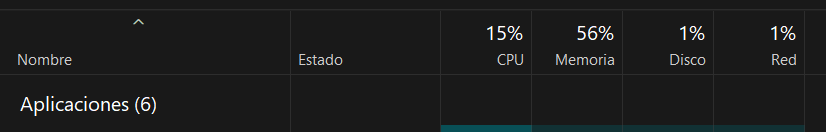
\includegraphics[width=0.75\textwidth]{Imagenes/Vectorial/6APPsNoOBS}
  \caption{Consumo del sistema sin OBS en ejecución: 15\,\% de CPU global y 56\,\% de memoria.}
  \label{fig:metric_noobs}
\end{figure}

\begin{figure}[H]
  \centering
  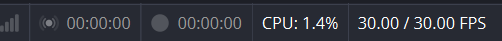
\includegraphics[width=0.75\textwidth]{Imagenes/Vectorial/6AppsSoloOBS}
  \caption{OBS Studio activo sin ningún filtro de realidad aumentada: 1,4\,\% de CPU reportado por OBS y cadencia estable de 30\,/\,30 fotogramas por segundo.}
  \label{fig:metric_soloobs}
\end{figure}

\subsection{Modo modelo 3D}
\label{sec:val_rend_3d}

El modo de modelo 3D es el de menor impacto computacional del sistema. Con un único filtro activo, OBS Studio consume un 1,1\,\% de CPU y 168,9\,MB de memoria, manteniendo la tasa objetivo de 30\,/\,30 fotogramas por segundo. La barra de estado de OBS reporta igualmente un 1,4\,\% de CPU.

Al escalar a tres filtros de modelo 3D activos simultáneamente sobre la misma escena, el consumo de CPU de OBS asciende al 2,2\,\% y la memoria crece hasta 228,8\,MB, manteniéndose en todo momento la cadencia de 30\,/\,30 fotogramas por segundo. Este resultado confirma que el coste del renderizado 3D con Assimp es muy reducido para modelos de complejidad moderada.

\begin{figure}[H]
  \centering
  \begin{minipage}{0.49\textwidth}
    \centering
    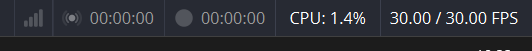
\includegraphics[width=\textwidth]{Imagenes/Vectorial/6APPSOBSModo3D_1modelo}
    \caption{Modo 3D con 1 filtro: 1,1\,\% de CPU y 168,9\,MB.}
    \label{fig:metric_3d_1}
  \end{minipage}\hfill
  \begin{minipage}{0.49\textwidth}
    \centering
    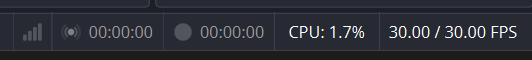
\includegraphics[width=\textwidth]{Imagenes/Vectorial/6APPSOBSModo3D_3modelos}
    \caption{Modo 3D con 3 filtros: 2,2\,\% de CPU y 228,8\,MB.}
    \label{fig:metric_3d_3}
  \end{minipage}
\end{figure}

\subsection{Modo AR con detección de marcadores}
\label{sec:val_rend_ar}

El modo AR, que incorpora la detección de marcadores ArUco en cada fotograma mediante OpenCV, representa la carga más intensiva del sistema. Con un único filtro activo, OBS reporta un 10,8\,\% de CPU y el Administrador de Tareas sitúa el proceso de OBS en un 12,3\,\% de CPU y 193,5\,MB de memoria, mientras la cadencia se mantiene estable en 30\,/\,30 fotogramas por segundo.

Sin embargo, al activar tres filtros AR simultáneos sobre la misma escena, el sistema supera su capacidad: la barra de OBS asciende al 26,5\,\% de CPU y la cadencia cae a 16,88\,/\,30 fotogramas por segundo, lo que representa una pérdida del 44\,\% de los fotogramas objetivo. El Administrador de Tareas sitúa el proceso de OBS en un 16,7\,\% de CPU y 272,5\,MB de memoria. Este límite es consecuencia directa de ejecutar tres instancias independientes del detector ArUco de OpenCV en el mismo hilo de renderizado, cada una procesando el fotograma completo en cada ciclo.

\begin{figure}[H]
  \centering
  \begin{minipage}{0.49\textwidth}
    \centering
    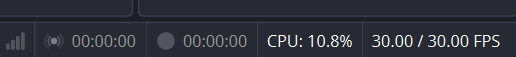
\includegraphics[width=\textwidth]{Imagenes/Vectorial/6APPSOBSModoAR_1filtro}
    \caption{Modo AR con 1 filtro: 12,3\,\% de CPU y 193,5\,MB, cadencia estable.}
    \label{fig:metric_ar_1}
  \end{minipage}\hfill
  \begin{minipage}{0.49\textwidth}
    \centering
    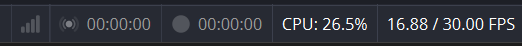
\includegraphics[width=\textwidth]{Imagenes/Vectorial/6APPSOBSModoAR_3filtros}
    \caption{Modo AR con 3 filtros: cadencia degradada a 16,88\,/\,30 fotogramas por segundo.}
    \label{fig:metric_ar_3}
  \end{minipage}
\end{figure}

\subsection{Modos marcador de clasificación e información de equipo}
\label{sec:val_rend_sb_ti}

Los modos de clasificación e información de equipo presentan un consumo intermedio, similar entre sí dado que ambos ejecutan la detección de marcadores (cuando la sincronización AR está activa) más el renderizado de texto.

El modo de clasificación sin sincronización AR consume un 10,4\,\% de CPU según OBS (11,3\,\% en el Administrador de Tareas) y 180,4\,MB de memoria, con cadencia estable de 30\,/\,30 fotogramas por segundo. Al activar la detección de marcadores en este mismo modo, el consumo sube ligeramente a 11,2\,\% (OBS) / 12,4\,\% (sistema) y 160,4\,MB, sin afectar a la cadencia.

El modo de información de equipo con detección de marcadores activa consume un 11,3\,\% de CPU (OBS) / 14,3\,\% (sistema) y 154,4\,MB de memoria, manteniendo igualmente los 30\,/\,30 fotogramas por segundo.

\begin{figure}[H]
  \centering
  \begin{minipage}{0.49\textwidth}
    \centering
    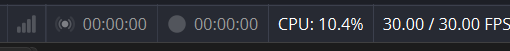
\includegraphics[width=\textwidth]{Imagenes/Vectorial/6APPsOBSModoScoreboardNoAruko}
    \caption{Modo marcador de clasificación sin detección ArUco: 11,3\,\% de CPU.}
    \label{fig:metric_sb_noar}
  \end{minipage}\hfill
  \begin{minipage}{0.49\textwidth}
    \centering
    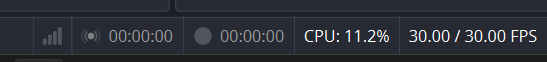
\includegraphics[width=\textwidth]{Imagenes/Vectorial/6APPSOBSModoScoreboardConAruco}
    \caption{Modo marcador de clasificación con detección ArUco activa: 12,4\,\% de CPU.}
    \label{fig:metric_sb_ar}
  \end{minipage}
\end{figure}

\begin{figure}[H]
  \centering
  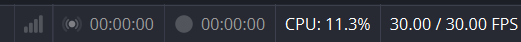
\includegraphics[width=0.75\textwidth]{Imagenes/Vectorial/6APPSOBSModoTeamInfoAruco}
  \caption{Modo información de equipo con detección ArUco: 14,3\,\% de CPU y 154,4\,MB, cadencia estable de 30\,/\,30.}
  \label{fig:metric_teaminfo}
\end{figure}

\subsection{Uso simultáneo de múltiples filtros}
\label{sec:val_rend_multimode}

Para evaluar el comportamiento en escenarios de producción real, donde puede ser necesario aplicar el complemento en varias fuentes de cámara simultáneamente, se midió el consumo con una configuración mixta de tres filtros: un filtro en modo clasificación y dos filtros en modo información de equipo, todos con detección de marcadores activa.

Bajo esta configuración, OBS reporta un 25,1\,\% de CPU y la cadencia cae a 16,45\,/\,30 fotogramas por segundo. El Administrador de Tareas sitúa el proceso de OBS en un 22,7\,\% de CPU y 270,9\,MB de memoria. Al igual que en el caso de tres filtros AR, la degradación de la tasa de fotogramas se debe a que cada filtro ejecuta su propia instancia del detector ArUco en el hilo de renderizado, multiplicando la carga de visión artificial por el número de filtros activos.

\begin{figure}[H]
  \centering
  \begin{minipage}{0.49\textwidth}
    \centering
    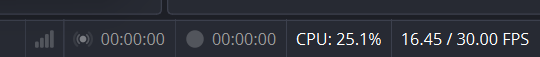
\includegraphics[width=\textwidth]{Imagenes/Vectorial/6APPSOBS_MIX_1SCOREBOARD2TEAMINFO}
    \caption{Configuración mixta (1 marcador de clasificación + 2 información de equipo): OBS reporta 25,1\,\% de CPU.}
    \label{fig:metric_mix_obs}
  \end{minipage}\hfill
  \begin{minipage}{0.49\textwidth}
    \centering
    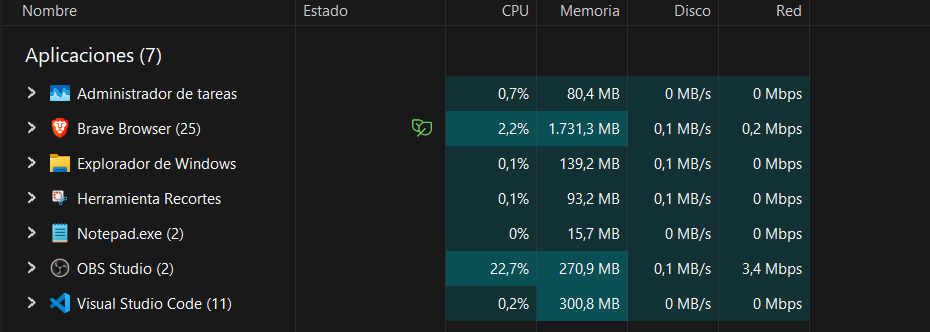
\includegraphics[width=\textwidth]{Imagenes/Vectorial/6APPSOBS_MIXED1COREBOARD2TEAMINFO_2}
    \caption{Administrador de Tareas bajo la configuración mixta: 22,7\,\% de CPU y cadencia degradada a 16,45\,/\,30.}
    \label{fig:metric_mix_sys}
  \end{minipage}
\end{figure}

\subsection{Resumen de resultados}
\label{sec:val_resumen}

La tabla~\ref{tab:metricas_rendimiento} recoge de forma consolidada los resultados de todas las mediciones realizadas.

\begin{table}[H]
\centering
\small
\begin{tabularx}{\textwidth}{l c c c}
\toprule
\textbf{Configuración} & \textbf{CPU OBS (\%)} & \textbf{Memoria OBS (MB)} & \textbf{Fotogramas/s} \\
\midrule
OBS sin filtros               & 1,4  & n/d   & 30\,/\,30 \\
Modo 3D, 1 filtro             & 1,1  & 168,9 & 30\,/\,30 \\
Modo 3D, 3 filtros            & 2,2  & 228,8 & 30\,/\,30 \\
Modo AR, 1 filtro             & 12,3 & 193,5 & 30\,/\,30 \\
Modo AR, 3 filtros            & 16,7 & 272,5 & 16,88\,/\,30 \\
Scoreboard (sin ArUco)        & 11,3 & 180,4 & 30\,/\,30 \\
Scoreboard (con ArUco)        & 12,4 & 160,4 & 30\,/\,30 \\
Info equipo (con ArUco)       & 14,3 & 154,4 & 30\,/\,30 \\
Mixto: 1 Scoreboard + 2 Info  & 22,7 & 270,9 & 16,45\,/\,30 \\
\bottomrule
\end{tabularx}
\caption{Resumen de consumo de CPU, memoria y tasa de fotogramas por configuración.}
\label{tab:metricas_rendimiento}
\end{table}

Los resultados permiten extraer las siguientes conclusiones:

El modo de modelo 3D puro tiene un impacto prácticamente nulo sobre el sistema y escala con normalidad al usar varios filtros simultáneos. Los modos que incorporan detección de marcadores ArUco representan un coste de CPU de entre el 10\,\% y el 14\,\% por filtro, pero un único filtro activo mantiene siempre la cadencia objetivo de 30 fotogramas por segundo. El límite práctico del sistema aparece al activar tres o más filtros con detección de marcadores simultáneos: en ese escenario la cadencia cae por debajo de 20 fotogramas por segundo, lo que resulta perceptible en la retransmisión. Este comportamiento es consistente con la arquitectura actual, en la que cada filtro ejecuta OpenCV de forma independiente. Una optimización futura que compartiera una única instancia del detector entre todos los filtros activos podría reducir significativamente este coste.
